\documentclass{beamer}

\usepackage[utf8]{inputenc}
\usepackage[T1]{fontenc}
\usepackage[english]{babel}
\usepackage{tikz}
\usepackage{algorithm}
\usepackage{algorithmicx}
\usepackage{algpseudocode}
\usepackage{amsmath}
\usepackage{caption}
\usepackage{subcaption}

\usetheme{default}

\newcommand{\bigO}[1]{\mathcal O \left( #1\right)}
\newcommand{\F}[0]{\mathcal{F}}
\newcommand{\SymF}[0]{\mathcal{S}ym\mathcal{F}}
\newcommand{\LitS}[0]{\mathcal{L}it\mathcal{S}}
\newcommand{\SymS}[0]{\mathcal{S}ym\mathcal{S}}
\newcommand{\Seeds}[0]{\mathcal{S}eeds}
\newcommand{\N}[0]{\mathcal{N}}
\newcommand{\A}[0]{\mathcal{A}}


\title{MPRI 2.19 - Programming project}
\subtitle{Analysis of cyclic attractors for \\ asynchronous boolean models of cellular networks}
\author{Marc Heinrich \and Baptiste Lefebvre}
\institute{École Normale Supérieure, Computer Science Department}
\date{February 24, 2015}


% README
% 
% Soutenance mardi 24 février entre 09h30 et 11h30.
% 
% Objectif:
%   - présenter le projet de programmation
%   - présenter qui a fait quoi pour la réalisation du projet
%   - présenter les résultats obtenus
%
% Durée:
%   - 25 minutes de présentation
%   - 15 minutes de questions


\begin{document}


\section*{Title}

\begin{frame}
  \titlepage
\end{frame}


\section*{Table of contents}

\begin{frame}
  \frametitle{Table of contents}
  \tableofcontents
\end{frame} 


% Presentation %%%%%%%%%%%%%%%%%%%%%%%%%%%%%%%%%%%%%%%%%%%%%%%%%%%%%%%%%%%%%%%%%

\section{Presentation}

\begin{frame}
  \frametitle{Presentation}    
  \begin{figure}
    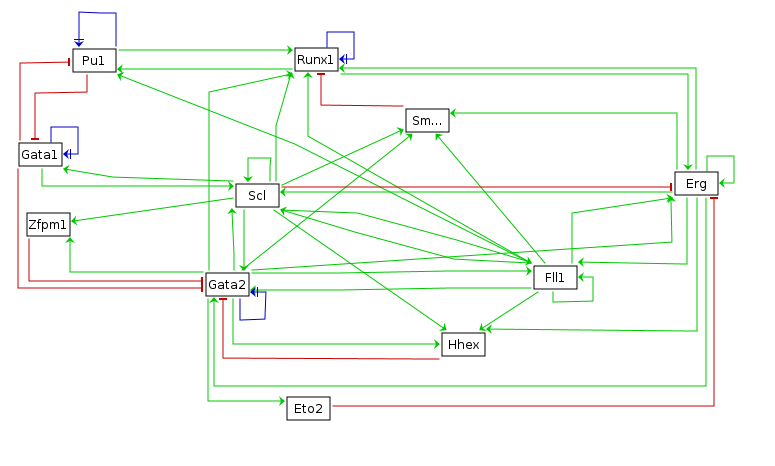
\includegraphics[scale=0.4]{img/hematopoietic}
    \caption{Boolean Model for blood stem cells \cite{Bonzanni}}
  \end{figure}
\end{frame}

% Maybe not put here
% Slides from previous presentation
\begin{frame}
  % 2 minutes... probably 3 actually
  \frametitle{BDDs/MDDs}
  Compact representation of a boolean function with $ n $ variables
  
  \begin{figure}
    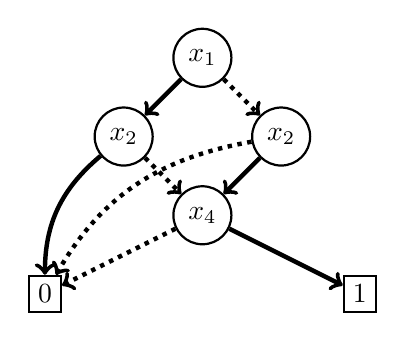
\begin{tikzpicture}
      \tikzstyle{endnode} = [draw, rectangle, thick, black] ;
      \tikzstyle{varnode} = [draw, circle, thick, black] ;
      \tikzstyle{onearrow} = [->, ultra thick, black] ;
      \tikzstyle{zeroarrow} = [->, ultra thick, black, dotted] ;
      \node[varnode] (x1) at (0,0) {$x_1$} ;
      \node[varnode] (1x2) at (-1,-1) {$x_2$} ;
      \node[varnode] (2x2) at (1,-1) {$x_2$} ;
      \node[varnode] (x4) at (0,-2) {$x_4$} ;
      \node[endnode] (1) at (2,-3) {1} ; 
      \node[endnode] (0) at (-2,-3) {0} ;
      \draw[onearrow] (x1) -- (1x2) ;
      \draw[onearrow] (1x2) to[out=-140, in=90] (0) ;
      \draw[onearrow] (x4) -- (1) ;
      \draw[onearrow] (2x2) -- (x4) ;
      \draw[zeroarrow] (x1) -- (2x2) ;
      \draw[zeroarrow] (2x2) to[out=-170, in = 60] (0) ;
      \draw[zeroarrow] (1x2) -- (x4) ;
      \draw[zeroarrow] (x4) -- (0) ;
    \end{tikzpicture}
  \end{figure}

  \begin{definition}
    MDD : Extension to multivalued variables
  \end{definition}
\end{frame}

\begin{frame}
  \frametitle{Operations on MDDs}
  \begin{itemize}
  \item Apply binary operators (ex: AND, OR, EQUAL, ....)
    \bigskip
  
  \item Apply existential/universal quantifiers
    \bigskip
  
  \item Substitute variables
    \bigskip
  
  \item Composition of functions
    \bigskip
  
  \item Comparison of MDDs
    \bigskip
  
  \item Find satisfying assignments
  \end{itemize}
\end{frame}

\begin{frame}
%Mettre l'intérêt de cette structure de données
  \begin{block}{Pros}
    \begin{itemize}
    \item Compact representation of Boolean/Integer functions
    \item Represent a set of states by its indicator function.
    \end{itemize}
  \end{block}
  
  \bigskip
  \begin{block}{Cons}
    \begin{itemize}
    % TODO: translate
    \item Of potentially exponential size
    % TODO: translate
    \item The size depends on the order of variables
    \end{itemize}
  \end{block}
\end{frame}


% Distribution of tasks %%%%%%%%%%%%%%%%%%%%%%%%%%%%%%%%%%%%%%%%%%%%%%%%%%%%%%%%

\section{Distribution and description of tasks}

\begin{frame}
% 1 minute
  \frametitle{Distribution of tasks} 
  Implementation of different modules for GINsim
  \bigskip
  
  \begin{itemize}
  \item Finding minimum perturbation (Marc)
    \bigskip
    
  \item MDD based algorithm for computing attractors (Marc)
    \bigskip
    
  % TODO : better description
  \item LIP based algorithm for computing attractors (Baptiste)
  \end{itemize}
\end{frame}


\subsection{Minimum perturbation}

\begin{frame}
  % 2- minutes
  % explain problem
  \frametitle{Finding the minimum perturbation}
  \begin{block}{Problem}
    Given a set of initial states, find the minimum perturbation that allows to reach a given target state.
    
    Reformulation : among the ancestors of the target state, find the closest to the source.
  \end{block}
\end{frame}

\begin{frame}
  % TODO: explain example Bonzanni
  \begin{figure}
    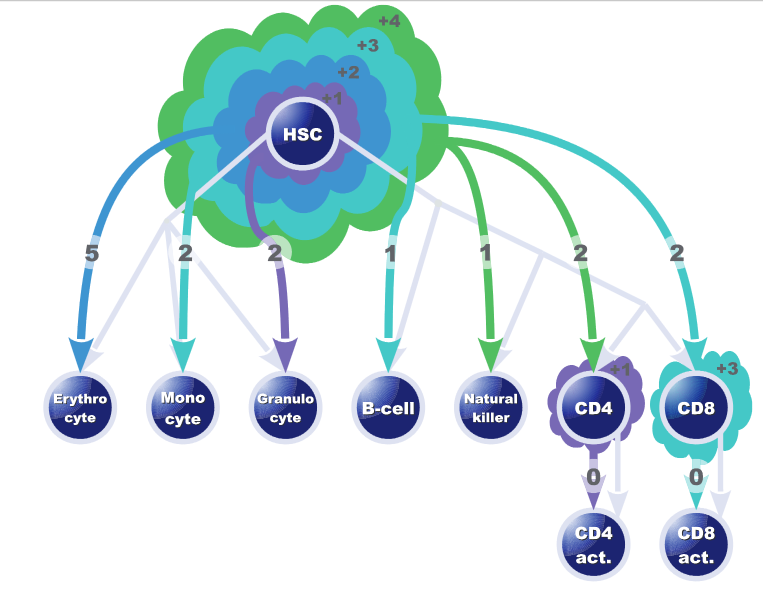
\includegraphics[scale=0.35]{img/push}
    \caption{Minimum perturbations for the model from Bonzanni et al.}
  \end{figure}
\end{frame}

\begin{frame}
  \frametitle{Solution}
  \begin{itemize}
  \item Compute the set of ancestors of the target state.
    \bigskip
    
  \item Enumerate all these states to find the closest.
  \end{itemize}
  \bigskip
  
  \onslide<2>
  \begin{block}{Improvement}
    Use only MDDs to compute the minimum number of genes to modify.
  \end{block}
\end{frame}


\subsection{Attractors via MDD}

\begin{frame}
% 3-4 minutes
  \frametitle{Finding attractors}
  \begin{definition}
    An attractor is a set of states that has no outbound transition, minimal for inclusion.
  \end{definition}
\end{frame}

\begin{frame}
  \frametitle{MDD formulation}
  \begin{block}{}
    Given a model, we represent it using MDDs by its transition function $f$:
    $$ f(x,y) =1 \Leftrightarrow x \rightarrow y$$
  \end{block}
  
  \begin{block}{Successor}
    The successors of a set of state $s(x)$ are the states $y$ that satisfy the MDD:
    $$ \exists x, s(x) \wedge f(x,y)$$
  \end{block}
  
  \begin{block}{Predecessor}
    The predecessors of a set of state $s(y)$ are the states $x$ that satisfy the MDD:
    $$ \exists y, s(y) \wedge f(x,y)$$
  \end{block}
\end{frame}

\begin{frame}
  %Synchronous algorithm
  \frametitle{Synchronous algorithm}
  
  \begin{block}{Notations}
    \begin{itemize}
    \item $FR(x) = \{ y,  x \rightarrow^* y \}$ : descendants of $x$
    \item $BR(x) = \{ y, y \rightarrow^* x \} $ : ancestors of $x$
    \end{itemize}
  \end{block}
  
  \bigskip
  \begin{algorithmic}
    \State $states \gets \mathcal S$
    \State $Att_{syn} \gets \emptyset$
    \While{$states \neq \emptyset$}
      \State $x \gets \text{FindState}(states)$
      \State $Att_{syn}.add(FR(x))$
      \State $states \gets states \setminus BR(x)$
    \EndWhile
  \end{algorithmic}
  
\end{frame}

\begin{frame}
  \frametitle{Asynchronous algorithm}
  %Asynchronous algorithm
  
  \begin{block}{Property}
    A state $x$ is in an attractor $\Leftrightarrow FR(x) \subseteq BR(x)$ 
  \end{block}
  
  \bigskip
  \begin{algorithmic}
    \State $states \gets \mathcal{S}$
    \State $Att_{asyn} \gets \emptyset$
    \While{$states \neq \emptyset$} 
      \State Take $s \in states$ 
      \If{$FR_{asyn}(s) \subset BR_{asyn}(s)$}
        \State $Att_{asyn}.add(FR_{asyn}(s))$ 
      \EndIf 
      \State $states \gets states \setminus BR_{asyn}(s)$
    \EndWhile
  \end{algorithmic}
\end{frame}

\begin{frame}
  \frametitle{Attractors classification}
  \begin{figure}
    \centering
    \begin{subfigure}[t]{0.3\textwidth}
      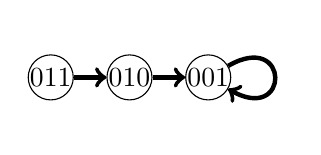
\begin{tikzpicture}
	\tikzstyle{node} = [draw, circle, black, inner sep = 0pt] ;
	\tikzstyle{arrow} = [->, ultra thick, black] ;
	\node[node] (a) at (0,0) {011}  ;
	\node[node] (b) at (1,0) {010} ;
	\node[node] (c) at (2,0) {001} ;
	\draw[arrow] (a) -- (b) ;
	\draw[arrow] (b) -- (c) ;
	\draw[arrow] (c) to[out= 30, in =-30, looseness =8] (c) ;
      \end{tikzpicture}
      \caption{Loop}
    \end{subfigure} 
    \qquad 
    \begin{subfigure}[t]{0.3\textwidth}
      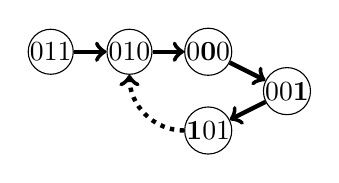
\begin{tikzpicture}
	\tikzstyle{node} = [draw, circle, black, inner sep=0pt] ;
	\tikzstyle{arrow} = [->, ultra thick, black] ;
	\node[node] (a) at (0,0) {011}  ;
	\node[node] (b) at (1,0) {010} ;
	\node[node] (c) at (2,0) {0\textbf{0}0} ;
	\node[node] (d) at (3,-0.5) {00\textbf{1}} ;
	\node[node] (e) at (2,-1) {\textbf{1}01} ;
	\draw[arrow] (a) -- (b) ;
	\draw[arrow] (b)-- (c) ;
	\draw[arrow] (c) -- (d) ;
	\draw[arrow] (d) -- (e) ;
	\draw[arrow, dotted] (e) to[out=180, in =-90] (b) ; 
      \end{tikzpicture}
      \caption{Simple cycle}
    \end{subfigure}
    
    \vspace*{0.5cm} 
    \begin{subfigure}[b]{0.3\textwidth}
      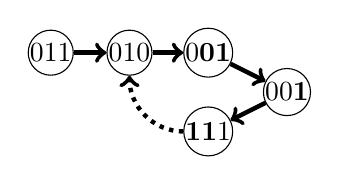
\begin{tikzpicture}
	\tikzstyle{node} = [draw, circle, black, inner sep=0pt] ;
	\tikzstyle{arrow} = [->, ultra thick, black] ;
	\node[node] (a) at (0,0) {011}  ;
	\node[node] (b) at (1,0) {010} ;
	\node[node] (c) at (2,0) {0\textbf{01}} ;
	\node[node] (d) at (3,-0.5) {00\textbf{1}} ;
	\node[node] (e) at (2,-1) {\textbf{11}1} ;
	\draw[arrow] (a) -- (b) ;
	\draw[arrow] (b)-- (c) ;
	\draw[arrow] (c) -- (d) ;
	\draw[arrow] (d) -- (e) ;
	\draw[arrow, dotted] (e) to[out=180, in =-90] (b) ; 
      \end{tikzpicture}
      \caption{Complexe synchronous cycle}
    \end{subfigure}
    \qquad 
    \begin{subfigure}[b]{0.3\textwidth}
      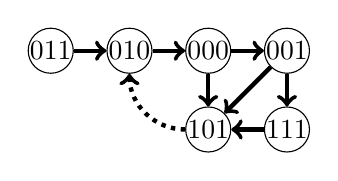
\begin{tikzpicture}
	\tikzstyle{node} = [draw, circle, black, inner sep=0pt] ;
	\tikzstyle{arrow} = [->, ultra thick, black] ;
	\node[node] (a) at (0,0) {011}  ;
	\node[node] (b) at (1,0) {010} ;
	\node[node] (c) at (2,0) {000} ;
	\node[node] (d) at (3,0) {001} ;
	\node[node] (e) at (2,-1) {101} ;
	\node[node] (f) at (3,-1) {111} ;
	\draw[arrow] (a) -- (b) ;
	\draw[arrow] (b)-- (c) ;
	\draw[arrow] (c) -- (d) ;
	\draw[arrow] (d) -- (e) ;
	\draw[arrow] (c) -- (e) ;
	\draw[arrow] (f) -- (e) ;
	\draw[arrow] (d) -- (f) ;
	\draw[arrow, dotted] (e) to[out=180, in =-90] (b) ; 
      \end{tikzpicture}
      \caption{Complex asynchronous cycle}
    \end{subfigure}
    \caption{All the possible attractors. (c) do not appear in the synchronous case, and (d) do not appear in the asynchronous case}
  \end{figure}
\end{frame}


\subsection{Attractors via ILP}

\begin{frame}
  \frametitle{Toward ILP formulation (I)}
  \begin{block}{Boolean network $ (V, F) $}
    \begin{itemize}
      \item $ V = \{ v_1, \cdots, v_n \} $ : variables
      \item $ F = \{ f_1, \cdots, f_n \} $ : boolean expressions over $ V $
    \end{itemize}
  \end{block}
  \pause
  \begin{block}{State transition graph $ (S, \rightarrow) $}
    \begin{overlayarea}{6cm}{4cm}
      \begin{itemize}
      \item $ S = \{ s : V \longrightarrow \mathbb{B} \} $ : state space
      \item $ F(s) = t $ \\
        where $ \forall v_i \in V, \; t(v_i) = f_i(s) $
      \item $ \rightarrow \; \subseteq \; S \times S $ : transitions
        \pause
        \begin{itemize}
          \setlength{\abovedisplayskip}{-11pt}
          \setlength{\belowdisplayskip}{0pt}
          \setlength{\abovedisplayshortskip}{0pt}
          \setlength{\belowdisplayshortskip}{0pt}
          \only<1>{\item pause 1}
          \only<2>{\item pause 2}
          \only<3>{
          \item synchronous transitions \\
            \begin{align*}
              \rightarrow_s = & \{ \left( s, t \right) \mid s \in S, \; t \in S, \; F(s) = t \} &
            \end{align*}
          }
          \only<4>{
          \item asynchronous transitions \\
            \begin{align*}
              \rightarrow_a = \{ \left( s, s \right) \mid & s \in S, \; F(s) = s \} & \\
              \cup \{ (s, t) \mid & s \in S, \; t \in S, \; \Delta(s, t) = 1, & \\
              & \Delta(t, F(s)) < \Delta(s, F(s)) \} &
            \end{align*}
          }
          \only<5>{
          \item $ \cdots $
          }
        \end{itemize}
      \end{itemize}
    \end{overlayarea}
  \end{block}
\end{frame}

\begin{frame}
  \frametitle{Toward ILP formulation (II)}
  \begin{block}{Literal}
    \begin{itemize}
    \item $ S = \{ s : V \rightarrow \mathbb{B} \} $ : state space
    \item $ F(s) = t $ \\
      where $ \forall v_i \in V, \; t(v_i) = f_i(s) $
    \item $ \F = \{ s \in S \mid F(s) = s \} $ : fixpoints
    \end{itemize}
  \end{block}
  \pause
  \begin{block}{Symbolic}
    \begin{itemize}
    \item $ SimS = \{ p : U_p \rightarrow \mathbb{B} \mid U_p \subseteq V \} $ : symbolic state space
    \item $ F[p] = q $ \\
      where $ U_q = \{v_i \in V \mid f_i[p] \in \mathbb{B} \} $ \\
      and $ \forall v_i \in U_q, \; q(v_i) = f_i[p] $
    \item $ \SymF = \{ p \in SimS \mid F[p] = p \} $ : symbolic fixpoints
    \end{itemize}
  \end{block}
\end{frame}

\begin{frame}
  \frametitle{Toward ILP formulation (III)}
  \begin{block}{Relaxed symbolic}
    \begin{itemize}
      \item $ \geq \quad \subseteq \; SimS \times SimS $ \\
        \begin{center}
          $ p \geq q \quad \Leftrightarrow \quad \begin{cases} p \; \text{and} \; q \; \text{are consistent} \\ U_p \supseteq U_q \end{cases} $
        \end{center}
      \item $ \Seeds = \{ p \in SimS \mid F[p] \geq p \} $ : seeds
    \end{itemize}
  \end{block}
  \pause
  \begin{block}{Trap set}
    $ R \subseteq S \; \text{is a trap set} \quad \Leftrightarrow \quad \begin{cases} R \neq \varnothing \\ \forall r, s \in R \times S, \; r \rightarrow s \Rightarrow s \in R \end{cases} $
  \end{block}
\end{frame}

\begin{frame}
  \frametitle{Central theorem}
  \begin{block}{Motivation}
    An inclusion-wise minimal trap set is also called an \emph{attractor} (i.e. \emph{steady state} or \emph{cyclic attractor})
  \end{block}
  \pause
  \begin{theorem}
    If $ p \in \Seeds $, then $ S[p] $ is a trap set in $ (S, \rightarrow_s) $  and in $ (S, \rightarrow_a) $
  \end{theorem}
  \pause
  \begin{proof}
    On the blackboard...
  \end{proof}
\end{frame}

\begin{frame}
  \frametitle{Consequences}
  \begin{center}
    \begin{equation*}
      \F \subseteq max(\SymF) = max(\Seeds) \subseteq \SymF \subseteq \Seeds
    \end{equation*}
    \bigskip
    \begin{equation*}
      \forall p \in max(\Seeds), \; S[p] \; \text{contains at least one attractor}
    \end{equation*}
  \end{center}
\end{frame}

\begin{frame}
  \frametitle{Translation (I)}
  \begin{block}{Prime implicant}
    \begin{equation*}
      p \in SymS \; \text{is a c-prime implicant of} \; f_i \notin \mathbb{B} \quad \Leftrightarrow \quad \begin{cases} f[p] = c \in \mathbb{B} \\ \forall q < p, \; f[q] \neq c \end{cases}
    \end{equation*}
    \begin{equation*}
      p \in SymS \; \text{is a c-prime implicant of} \; f_i \in \mathbb{B} \quad \Leftrightarrow \quad \begin{cases} U_p = v_i \\ p(v_i) = c \end{cases}
    \end{equation*}
  \end{block}
\end{frame}

\begin{frame}
  \frametitle{Translation (II)}
  \begin{block}{Prime implicant graph $ (\N, \A) $}
    \begin{itemize}
      \item $ \N = \{ p \in \SymS \mid |U_p| = 1 \} $
      \item
        \begin{align*}
          \A = \left\{ \left( \{ p_1, \cdots, p_{|p|} \}, \{ q \} \right) \mid \right. & \exists c \in \mathbb{B}, \; \exists v_i \in V, \\
          & p \; \text{is a c-prime implicant of} \; f_i, \\
          & U_q = \{ v_i \}, \; q(v_i) = c \}
        \end{align*}
    \end{itemize}
  \end{block}
  \begin{block}{Consistent arc set}
  \end{block}
  \begin{block}{Stable arc set}
  \end{block}
\end{frame}

\begin{frame}
  \frametitle{Translation theorem}
  \begin{theorem}
    $ p \in \Seeds $ if and only if there is a stable and consistent $ A \in \mathcal{A} $ such that $ H(A) = p $
  \end{theorem}
  \begin{proof}
    See \cite{Klarner}
  \end{proof}
\end{frame}

\begin{frame}
  \frametitle{Consequences}
  \begin{itemize}
    \item Straightforward translation of seeds into arc sets (i.e. prime implicant sets)
    \item Obvious 0-1 optimization problem to compute the maxima of these sets (i.e. trap sets)
    \item Natural reformulation as linear 0-1 inequalities (with \emph{Oj! Algorithm} or \emph{OjAlgo})
  \end{itemize}
\end{frame}


% Results %%%%%%%%%%%%%%%%%%%%%%%%%%%%%%%%%%%%%%%%%%%%%%%%%%%%%%%%%%%%%%%%%%%%%%

\section{Results}

\begin{frame}
  \frametitle{Results}
  \begin{center}
    Demonstration on GINsim of the different plugins
  \end{center}
  % TODO: add performance table if necessary
\end{frame}


\section*{References}

\begin{frame}
  \frametitle{References}
  \bibliographystyle{apalike}
  \bibliography{presentation.bib}
\end{frame}


\end{document}
